\section{Session 15. Integer programming}

material: cuttingstock.pdf

\begin{itemize}
  \item Getting familiar with the use of integer programming
  \item Solving integer programming problems
\end{itemize}

\begin{itemize}
  \item Problems in which the feasible set is composed of only integer values.
  \item The feasible set is neither continuous nor feasible.
  \item NP-hard problems in general.
  \item Integer problems that have a network structure are easy to solve using the Simplex method (assignment and matching problems, transportation and transshipment problems, and network flow problems always produce integer results, provided that the problem bounds are integers).
  \item Rounding can be effective in some problems and clearly not in others:
  \begin{itemize}
    \item not the same tires than aircrafts!
    \item values 0/1 for variable: zero-one or binary integer programming (produce or not produce cars in this factory)
    \item mixed integer programming problems
  \end{itemize} 
\end{itemize}


  \begin{equation*}
    \begin{aligned}
      \text{maximize } \quad & \sum_{j=1}^{n} c_j x_j \\
      \text{subject to }\quad &
      \begin{array}{rcl}
        \sum_{j=1}^n a_{ij} x_j= b_i&i=1,2,\ldots,m&  \\
        x_j > 0 &j=1,2,\ldots,n&\\
        x_j \quad \mathrm{integer} & \mathrm{for\,some\,or\,all\,} & j=1,2,\ldots,n
      \end{array}
    \end{aligned}
  \end{equation*}



    \begin{center}
      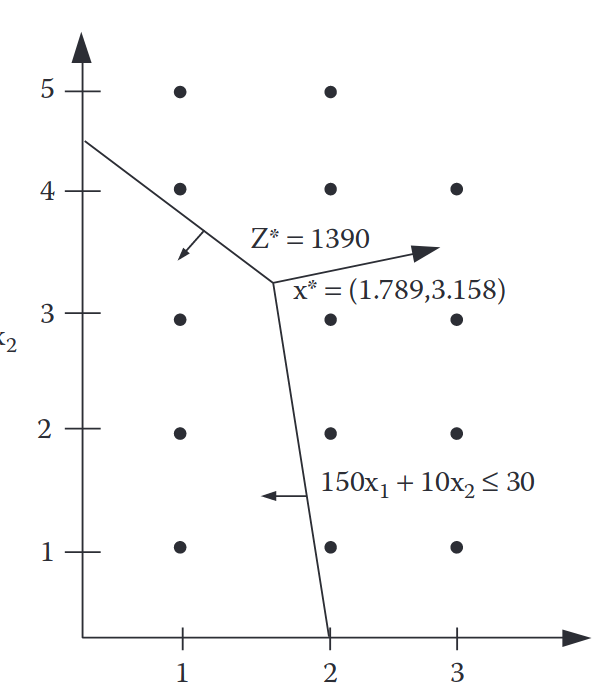
\includegraphics[width=0.4\linewidth]{../figures/IntegerProgramming.png}
    \end{center}
    Graphical representation of a typical 2 dimensional integer programming\cite{carter_operations_2019}.


  
    \begin{itemize}
      \item Capital budgeting: deciding between a collection of investiments
      \item Warehouse location: in modelling distribution systems, we should decide about tradeoffs between transportation costs and costs for operating distributions centers
      \item Scheduling: students-faculty-classrooms allocations, vehicle dispatching, etc (see next slide)
    \end{itemize}
  


  {\bf Airline crew scheduling problem}: The airlines first design a flight schedule composed of a large number of {\em flight legs} (specific flight on a specific piece of equipment, such as a 747 from New York to Chicago departing at 6:27 a.m.). A flight crew is a complete set of people, including pilots, navigator, and flight attendants who are trained for a specific airplane. A work schedule or rotation is a collection of flight legs that are feasible for a flight crew, and that normally terminate at the point of origin. Variables $x_{ij}$ have value 1 if flight leg $i$ is assigned to crew $j$. All flight legs should be covered at minimum total cost. 
  \\[10pt]
  Also called a {\em set-partitioning problem}
  \begin{equation*}
    \begin{aligned}
      \text{minimize } \quad & \sum_{j=1}^{n} c_j x_j \\
      \text{subject to }\quad &
      \begin{array}{rcl}
        \sum_{j=1}^n a_{ij} x_j= 1&i=1,2,\ldots,m&  \\
        x_j = {0,1} &j=1,2,\ldots,n
      \end{array}
    \end{aligned}
  \end{equation*}



  \begin{Exercise}
    Consider the travelling salesman problem. Starting from his home, a salesman wishes to visit each of $(n-1)$ other cities and return home at minimal cost. He must visit each city exactly once and the cost to travel from city $i$ to $j$ is $c_{ij}$. Let $x_{ij}$ be 1 or 0 depending on the fact that he goes or not from city $i$ to city $j$
    \begin{itemize}
      \item formulate the optimization problem
      \item how to avoid disjoint tours?
    \end{itemize}
  \end{Exercise}



  Simplex is not useful to solve, in general, integer problems. Instead, many other techniques have been proposed:
  \begin{itemize}
    \item Enumeration techniques, including the branch-and-bound procedure;
    \item cutting plane techniques; and 
    \item group-theoretic techniques,
  \end{itemize}

  as well as several composite techniques
  




    \begin{center}
      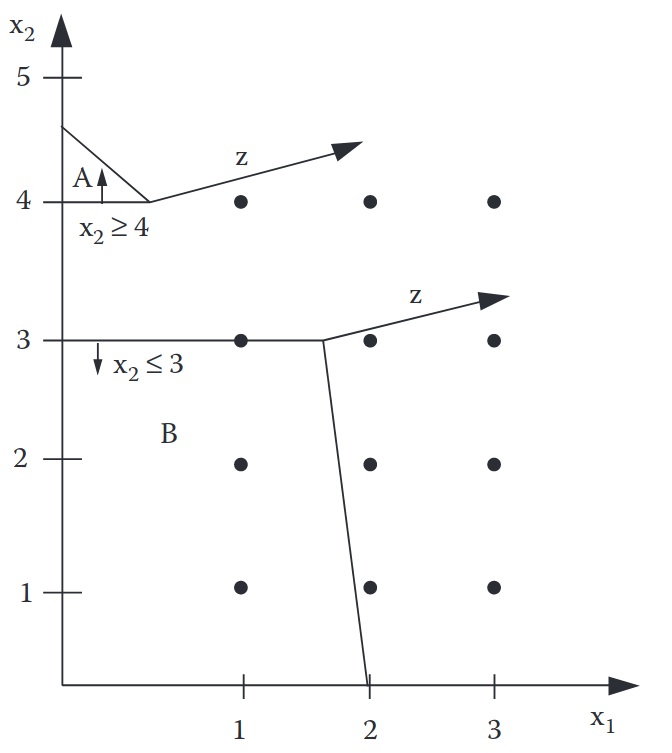
\includegraphics[width=0.4\linewidth]{../figures/BranchandBound.png}
    \end{center}
    Separation into two subproblems in the Branch-and-Bound method\cite{carter_operations_2019}.


  \begin{Exercise}
    Using the graphical representation and the branch-and-bound procedure, solve this integer program:
    \begin{equation*}
      \begin{aligned}
        \text{maximize } \quad & z=x_1+5x_2 \\
        \text{subject to }\quad &
        \begin{array}{rcl}
          -4x_1+3x_2\leq 6&&  \\
          3x_1+2x_2\leq 18&&  \\
          x_1,x_2 \geq 0 & \mathrm{and\,integer}
        \end{array}
      \end{aligned}
    \end{equation*}
  \end{Exercise}





